\documentclass{beamer}
\usetheme[block=fill]{metropolis}

\usepackage[english]{babel}
%\usepackage[utf8]{inputenc}

% For notes
\usepackage{pgfpages}
\setbeameroption{show notes on second screen=right}
\usepackage{appendixnumberbeamer} % don't number the backup slides

\usepackage{amsmath,amssymb} % math
\usepackage{graphicx} % images
\DeclareGraphicsExtensions{.eps,.pdf,.png,.jpg,.gif}
\graphicspath{{./img/}}

\title{aursec - A blockchain approach to securing software packages}
\author{Lukas Krismer \& Bennett Piater}
\institute{Universität Innsbruck - QE - Christian Sillaber}
\date{\today}

\begin{document}

\maketitle


\begin{frame}
	\frametitle{Outline}
	\tableofcontents
	\note{1 min L}
\end{frame}

\section{AUR}

\begin{frame}{AUR}
\begin{itemize}
	\item \textbf{AUR}=\alert{A}rch Linux \alert{U}ser \alert{R}epository
	\item Contains package build scripts (PKGBUILDs)
	\item Packages can be voted for inclusion in the official repositories
	\item Easy to use using so-called AUR helpers
	\item Everybody can upload PKGBUILDs
	\item Anyone can adopt orphaned packages
\end{itemize}
\note{2min L}
\end{frame}

\begin{frame}{Threat Assessment}
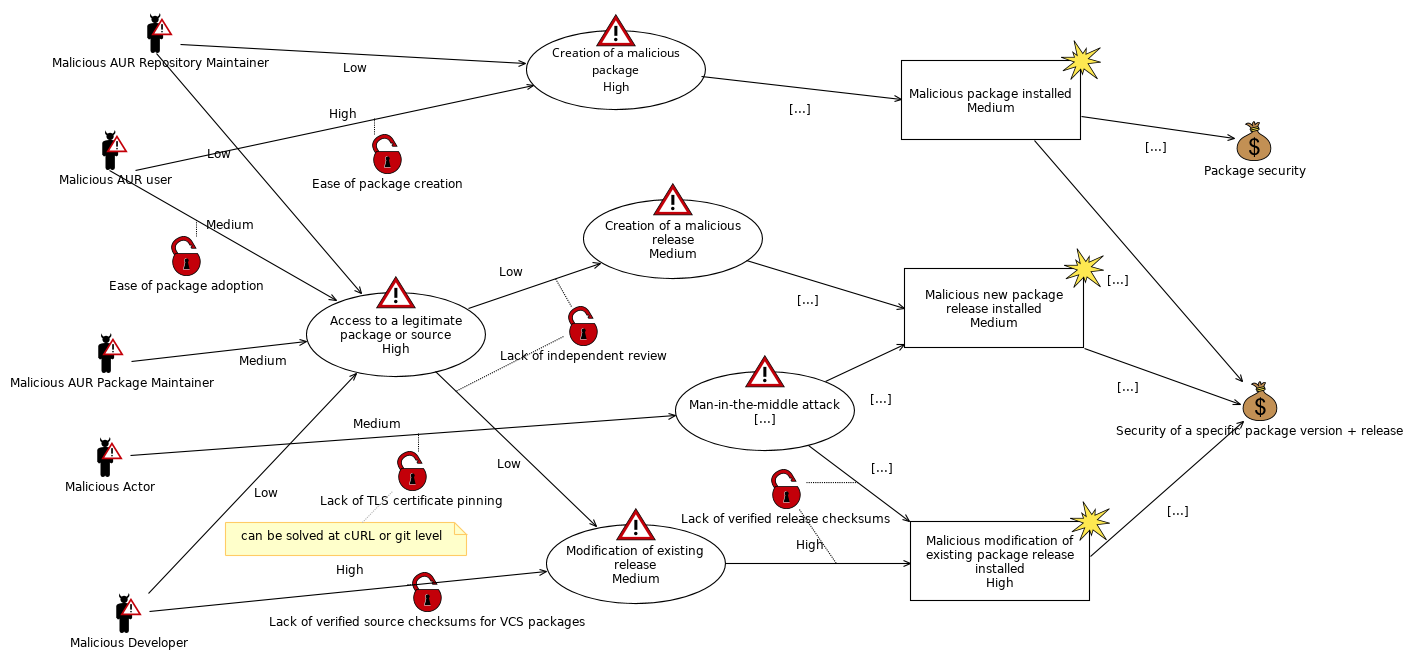
\includegraphics[width=\textwidth]{threat.png}
\note{2 min B | Besonderes Augenmerk auf:

\begin{itemize}
	\item Die grundlegenden Probleme der AUR sind praktisch unlösbar
	\item Zu viele haben Zugang zu Quellen und/oder Buildskripten
	\item Daher: Server-Seitige Signaturen würden nur MITM verhindern
	\item Bösartige Pakete, Releases oder Veränderungen sehr einfach
\end{itemize}}
\end{frame}

\section{Our Project}

\begin{frame}{Covered Threats}
\includegraphics<1>[width=\textwidth]{threat.png}
\includegraphics<2>[width=\textwidth]{threat2.png} 
\note{1 min L}
\end{frame}

\begin{frame}{Basic Workflow of the Core Library}
\begin{center}
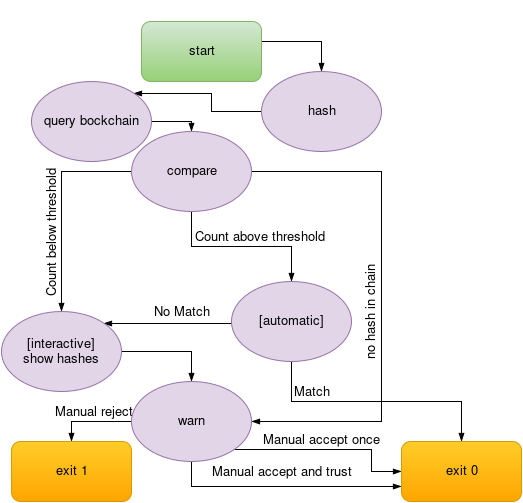
\includegraphics[height=0.9\textheight]{workflow.png}
\end{center}
\note{3 min L }
\end{frame}

\begin{frame}{Components}
\begin{itemize}
	\item Program on a private Ethereum blockchain
	\item Shell library
	\item AUR package
	\item Integration in aurutils
	\item Threat analysis of the AUR and our software
	\item Web- and/or CLI-Interface for stats/events
\end{itemize}
\note{2 min B

\begin{itemize}
	\item Das eigentliche Programm zum Speichern der Hashes
	\item Unsere Library, die den Workflow automatisiert
	\item Ein Paket für die AUR
	\item Integration in einen der Besten AUR-Helper \\
	--> Im Zuge dessen allgemein nützliche Beiträge dazu
    \item Threat-analysen, um die Gefährdungsstufe und die Qualität unseres Beitrags einzuschätzen
    \item Ein Interface, mit dem die Aktivität der Blockchain überwacht werden kann
\end{itemize}}
\end{frame}

\begin{frame}{Schedule}
\begin{itemize}
	\item \textbf{25.10} \emph{prototype:} hashing \hfill B
	\item \textbf{08.11} \alert{Initial Presentation}\hfill L
	\item \textbf{15.11} \emph{prototype:} library without blockchain back-end \hfill B/L
	\item \textbf{15.11} Bash-API for the blockchain \hfill L
	\item \textbf{30.11} \emph{finish:} \alert{Solidity program} \hfill B
	\item \textbf{08.12} deploy local blockchain for development \hfill L
	\item \textbf{08.12} running server with ethereum-node \hfill B/L
	\item \textbf{15.12} \emph{prototype:} \alert{Library} incl. back-end \hfill L
	\item \textbf{20.12} \emph{contrib:} pre-build-hooks in aurutils \hfill B
\end{itemize}
\note{2 min B

Wir haben eine sehr \textbf{detaillierte Planung} ausgearbeitet.
Einerseits benötigen wir sie, um effizient \textbf{kooperieren} zu können und zügig voran zu kommen; Andererseits soll sie uns auch ein Maximaltempo vergeben, denn wir tendieren beide eher dazu, uns zu \textbf{überarbeiten}.

\begin{itemize}
	\item Solidity-program auf Blockchain
	\item Library-Prototyp
	\item Beiträge zum AUR-Helper aurutils über Weihnachten
\end{itemize}
}
\end{frame}

\begin{frame}{Schedule}
\begin{itemize}
	\item \textbf{10.01} \emph{contrib:} TLS-public-key-pinning in aurutils \hfill B
	\item \textbf{10.01} configuration and trust-cutoff \hfill L
	\item \textbf{15.01} \emph{test:} \alert{Integration in aurutils} \hfill B
	\item \textbf{15.02} \alert{AUR package} incl. private blockchain \hfill B
	\item \textbf{01.03} \emph{finish:} libary and aurutils-Hook \hfill B
	\item \textbf{31.03} \emph{finish:} Web- and/or CLI-Interface \hfill L
	\item \textbf{21.04} \alert{Draft paper} for feedback\hfill
	\item \textbf{??.05} \emph{finish:} Paper\hfill
	\item \textbf{??.05} Final presentation\hfill L
\end{itemize}
\note{2 min B

\begin{itemize}
	\item am 15.01 mit aurutils testbar
	\item AUR-Paket zur einfachen Verbreitung
	\item Programmierung endet am 31. März
	\item Meiste Schreibarbeit im April und besonders über Ostern
	\item Abgabe bequem for den Klausuren
\end{itemize}}
\end{frame}


\end{document}
